% Note to self: Compile using BibTeX (not Biber!) and pdflatex (not xelatex!)

\documentclass[11pt,a4paper]{article}
\usepackage[hyperref]{acl2020}

 % times is deprecated - using a modern times clone instead
\usepackage{mathptmx}

%\usepackage{titlesec}
%\titleformat{\section}{\normalfont\bfseries}{\thesection}{1em}{}

\usepackage{lipsum}
\usepackage{amsmath,amsthm,amssymb}
\usepackage{graphicx}
\usepackage{latexsym}
\usepackage{booktabs}
\renewcommand{\UrlFont}{\ttfamily\small}

% This is not strictly necessary, and may be commented out,
% but it will improve the layout of the manuscript,
% and will typically save some space.
\usepackage{microtype}

\aclfinalcopy % Uncomment this line for the final submission
%\def\aclpaperid{***} %  Enter the acl Paper ID here

%\setlength\titlebox{5cm}
% You can expand the titlebox if you need extra space
% to show all the authors. Please do not make the titlebox
% smaller than 5cm (the original size); we will check this
% in the camera-ready version and ask you to change it back.

\title{PM Question Processing Final Project: 20 Questions}

\author{Wellesley Boboc \\
Universit{\"a}t Potsdam \\
Matriculation number: xxxxxx \\
\texttt{email@domain} \\\And
Anna-Janina Goecke \\
Universit{\"a}t Potsdam \\
Matriculation number: xxxxxx \\
\texttt{email@domain} \\\AND
Rodrigo Lopez Portillo Alcocer \\
Universit{\"a}t Potsdam \\
Matriculation number: xxxxxx \\
\texttt{email@domain} \\\And
Elizabeth Pankratz \\
Universit{\"a}t Potsdam \\
Matriculation number: xxxxxx \\
\texttt{email@domain} \\}

\date{}

\begin{document}
\maketitle

\begin{abstract}
\lipsum[1]
\end{abstract}

\section{Introduction: Task and motivation}

Our task is to build a system that will play the game 20 Questions (20Q).
A human player will be able to think of a target object, and the system will strategically select questions that allow it to narrow down the candidate objects in its knowledge base.
It will incorporate the answers it receives and ultimately make a guess about what that target object could be.
If the target object that the human player has in mind is not already in its knowledge base, the system will add it in based on the information the user has provided.

This task is interesting and challenging because it not only involves generating natural-language questions to present to the human player, but also choosing which questions are the best ones to ask, and manipulating the knowledge representation in accordance with the answers that the human player provides.

So, on the one hand, the project contains the computational-linguistic subtask of question generation (given a feature in the dataset, generate a natural-language question asking about that feature to display to the user), and on the other, the engineering subtask of knowledge base manipulation.
For the latter, we will need to strategically select the best question to ask, incorporate the answers from the user as the game is played, and at the end, add previously-unseen objects into the knowledge base.

\section{Related work}

We will briefly explore two areas in the literature that are relevant for our implementation: existing approaches to implementing 20Q, followed by rule-based question generation (QG).

\subsection{Previous 20Q implementations}

Previous approaches to the implementation of a 20Q system have made use of diverse methods including probabilistic models \citep{DeyEa2019}, Reinforcement Learning (RL; \citealt{HuEa2018}), and variations of Artificial Neural Networks (ANNs; \citealt{ReddyEa2017, Burgener2006, ToninEa2018}).
The knowledge that the 20Q system has is often represented in a knowledge graph (KG; \citealt{DeyEa2019}), though some more sophisticated approaches also manage without \citep[e.g.][]{HuEa2018}.%
\footnote{A KG is essentially a graph where the nodes are entities and the edges between them are facts that connect them.
	For instance, a node \textit{Macron} might be connected to a node \textit{Paris} by the edge \textit{lives in} \citep[example from][]{GodinEa2019}, representing knowledge of the fact \textit{Macron lives in Paris}.}
Here, we will briefly discuss the relative merits of these implementations and how they inform our work on this project.

We begin with some probabilistic approaches.
In general, these are characterised by maintaining a probability distribution over the set of outcomes.
Consequently, none of the possible outcomes are ever totally discounted or thrown away---just associated with a lower probability.
%These are often associated with Bayesian-style updating, where the probabilities are computed anew after every time step.
This approach is good for situations in which the questions are answered by the users in a ``noisy'' way (e.g.\ when users answer inconsistently or wrongly).
In those cases, the system is still able to choose what the correct target object might be, even though the user has answered in a way that might seem incompatible with that object.

\citet{DeyEa2019} implemented a probabilistic model which operates on the dataset as weighted edge-node relations of a KG and updates throughout the course of the game. 
Here, the main idea of adjusting probabilities at every time step was exploited to generate a model that is able to predict the correct target object in fewer than twenty questions. 
Of particular interest is the way the model handles incorrect answers from the human player: the question generator does not fully reject or accept a certain object as being the target after every answer. f
Instead, it rebalances the probabilities at each step in the game. 
To identify the target object, the model categorizes the questions into two layers, a primary layer (wide range of objects) and a secondary layer (specific range, targeted towards a small set of objects). 
Even though the model has been proven to perform very well, i.e.\ half of the target objects could be identified in fewer than ten questions, their work is very limited in that it is designed to only apply to Bollywood movies. 
However, the use of KGs to create 20Q (probably adapted from graph format into a tabular database; see below) is an approach that we would like to pursue for our 20Q implementation, by further elaborating the ideas of \citet{DeyEa2019}, among others.

\citet{HuEa2018} also rely on a probability distribution over all objects which is then updated according to the answers.
However, their approach is different in that they use an RL framework: they implement a policy-based system of 20Q that uses reinforcement throughout the game. 
Instead of using a KG, the model for selecting questions is based on RL procedures trying to find the optimal reward function. 
%The questioner agent relies on a probability distribution over all objects which is then updated according to the answers.
\citet{HuEa2018} suggest a neural network that they call RewardNet which learns the immediate reward at each time step to improve the overall performance of the model, since only receiving a reward at the end of the game wouldn't allow the system to learn for each question.
The model continually improved its win rate over time and was shown to be able to identify the target object within 14 questions.
While this system clearly has excellent performance, incorporating RL into our project is not feasible; it is included in this literature review only for the sake of completeness.

Another approach that is probably too sophisticated for us, but nevertheless useful to know about, is the use of neural networks.
For example, \citet{ReddyEa2017} propose the application of KGs to generate sets of question-answer pairs within a Recurrent Neural Network architecture by deriving triple relations from given entities. 
The triples are composed of a subject, an object (both represented as nodes in the KG), and a predicate (represented as an edge in the KG). 
The model consists of two units: the \textit{Question Keywords and Answer Extractor}, which directly selects necessary information about an object from the KG, and the \textit{Natural Language Question Generator}, which is used as an encoder and decoder of the object's representation. 
Since this model has been able to outperform comparable approaches on question generation, we could consider adapting some of the assumptions, such as deriving the triple relations of the KG, for our project implementation. 

Perhaps the most widely-known implementation of the 20Q game is that of \citet{Burgener2006}, which can be found at \url{20q.net} and is also a popular toy. 
With more than 88 million plays, Burgener's implementation has a precision rate of 80\% when it asks twenty questions, and 95\% for twenty-five questions. 
The patent for the game describes the implementation of the deep ANN, which is structured as a matrix of target objects by questions. 
Each cell of the matrix contains an input-output connection weight, which defines the relationship between the questions/answers and the target objects. 
The network has two so-called modes: the first takes questions as input and targets as output, and the second takes target objects as input nodes and questions as outputs. 
The first mode maps answers to weights, while the second mode ranks questions. 
Similar to \citet{DeyEa2019}, target objects are prioritized, rather than filtered. 
This is a primary motivation for Burgener's choice of architecture, as it allows the model to correctly predict the target even when given incorrect or inconsistent answers, as mentioned above. 
As Burgener explains, it also allows the system to take into account cultural/demographic differences that may result in inconsistent answers about a given target object. 
This is a consideration we should also be mindful of in our implementation, as our proposed model operates on the assumption that the user is providing truthful answers (and that inter-user agreement would be high). 
The system of weights also allows for a more complex set of inputs than binary yes/no (e.g.\ sometimes, maybe, depends, rarely) where the degree of certainty of the answer is reflected in the weights used. 
While our immediate plan is to implement a binary answering system (or perhaps a three-way system, where ``unsure/unknown'' could also be an answer that would not contribute to the machine's prediction) as a proof of concept, keeping degrees of certainty in mind may help us to improve our final implementation.

Finally, \citet{ToninEa2018} describe another ANN implementation of the 20Q framework as part of a brain-computer interface to enable people with motor impairments to communicate. 
The system uses a weight matrix to store the strength of the connection between target statements and questions (where negative weights indicate that the expected answer to the question is no, and vice-versa for positive weights). 
After 15 questions, the model checks to see if there is only one target statement with a positive value. 
If there is no single positive value after twenty questions, the network returns the statement with the highest current value. 
When the network correctly estimates the target, the weight matrix is updated. 
We may want to adopt this sort of ``early checking'' threshold before a final guess after twenty questions. 
This paper also presents a very interesting example of how a 20Q implementation may have useful applications outside of the realm of games and entertainment.

\subsubsection{Rule-based Question Generation}

In the field of QG, one of the approaches to generating syntactically coherent questions is based on finding rules. 
In our project, we would like to follow this rule-based approach, most likely using the spaCy\footnote{\url{https://spacy.io}} library, as we saw in class.
This is because questions in 20Q are syntactically limited, so we do not need more complex approaches for this task.

An interesting approach to rule-based QG is the work of \citet{MhatreEa2019}, which is based on keyword modelling using Named Entity Recognition (NER) to generate questions from an input sequence. 
Each input sentence is preprocessed and parsed to resolve anaphoric reference. 
Thereafter, NER is used to identify the type of entity, which is important for the choice of \textit{wh}-component for the QG part of the model. 
Depending on the output of the NER procedure, the appropriate \textit{wh}-pronoun is chosen. 
One type of questions they create are yes-no questions, which is the type of question we will focus on.
To construct this kind of question, the authors simply perform subject-auxiliary inversion. 
Since this work makes use of the spaCy architecture, it is of particular interest for this project.
In the case of NER, spaCy is a widely used structure that provides a large range of entity types. 

\citet{KhullarEa2018} concentrate on rule-based QG using relative pronouns to achieve high syntactic accuracy and semantic suitability. 
Their system uses the spaCy dependency parser to evaluate the syntactic structure of sentences. 
Firstly, the input sentence is parsed to gain information about the presence of relative pronouns and about several linguistic features. 
Afterwards, this information is input to one rule within a predefined rule set to create the questions. 
The correct \textit{wh}-component is then determined according to these rules, resulting in a syntactically coherent question. 

Both of the above-mentioned systems are fascinating in that they consist of a simple structure by using spaCy's dependency parser and NER methods. 
By further elaborating on these approaches, we should be able to construct simple yet appropriate yes-no questions for our 20Q model.

\section{Data}
We are currently developing the implementation on a preliminary knowledge base available \href{https://github.com/drdevinhopkins/20_Questions/blob/master/knowledge_base.csv}{here}.
It is a table consisting of 100 objects (mostly animals) and 28 features for each, and each cell in the table is populated with a 1 or a 0 to indicate that the given animal does or does not have the given feature.
For example, the first few rows and columns of the dataset look like this:

\begin{table}
\begin{center}
	\begin{tabular}{lccccc}
		\toprule
		Animal & Hair & Feathers & Eggs & Milk & \ldots \\ \midrule
		aardvark & 1 & 0 & 0 & 1 & \ldots \\
		antelope & 1 & 0 & 0 & 1 & \ldots \\
		bass & 0 & 0 & 1 & 0 & \ldots \\
		bear & 1 & 0 & 0 & 1 & \ldots \\
		boar & 1 & 0 & 0 & 1 & \ldots \\
		\vdots & \vdots & \vdots & \vdots & \vdots & $\ddots$ \\
		\bottomrule
	\end{tabular}
\end{center}
\caption{The first rows (instances) and columns (features) in our knowledge base}
\label{tab:knowledge-base}
\end{table}

Whichever dataset we end up actually using should be larger than this and have many more features, since the system is currently almost always able to finish within the 20-question limit.
We also found another promising dataset called Animals with Attributes\footnote{\url{https://cvml.ist.ac.at/AwA2/}} consisting of around 50 classes and 85 attributes. 
We are currently looking for larger open-source knowledge bases like this to use.

\section{Implementation}

[intro sentence]

\subsection{Probabilistic feature selection}

The machine learning system that we will use to implement this task is fairly simple: a decision tree (DT), also known as a CART model, which stands for ``classification and regression tree'' \citep[Section 16.2]{Murphy2012}.
A DT is ``defined by recursively partitioning the input space, and defining a local model in each resulting region of input space'' \citep[545]{Murphy2012}.
In our case, the input space consists of the knowledge base described above, and this knowledge base is recursively partitioned by each successive question that the system asks and the user answers.
However, in contrast to defining a local model in \textit{each} resulting region of input space, we will only retain the subset of the knowledge base that is compatible with the user's answers (at least, in the current, proof-of-concept stage of the project.
As we mentioned above, the benefits of using a more probabilistic approach are substantial, so we will likely end up going down that path as well, probably by simply strongly down-weighting the subset of the knowledge base that is incompatible with the user's answers).

In any case, we need to partition the space in an optimal way; how will we do this? 
Or in other words, how will we choose which question to ask?
One standard method in classification DTs splits the space on the feature that minimises the entropy (i.e.\ maximises the information gain; \citealt{Quinlan1986}), in each partition.
However, that method is not applicable here.
That method requires an $n : 1$ mapping of instances to each class, which is the usual set-up in classification problems: one class contains multiple instances.
In our task, though, each individual object equates to a class (i.e.\ there's an \textit{aardvark} class, an \textit{antelope} class, and so on), so there is only one instance per class.
That makes our problem a non-typical classification task, so a different method needs to be used.

We chose to orient ourselves around the size of the two partitions of the input space that result from splitting on a given feature, and we select the feature that produces the partitions that are closest to each other in size.
To illustrate, say that we split on the first feature given above, \textit{Hair}.
We would end up with one partition containing 57 animals that have no hair (i.e.\ where \textit{Hair} $= 0$), and another partition containing 43 animals with hair (i.e.\ where \textit{Hair} $= 1$).
To see how even this split is, we take a ratio of these two numbers.
We want this ratio to be as close to 1 as possible, since that would represent a perfect split of our input space in half: $\frac{50}{50} = 1$.
This is because since we only have two ``branches'' for each feature (yes or no, 1 or 0), consistently splitting our input space in half would result in the highest information gain regarding the class label. 
We selected this approach based on tree-based algorithms such as ID3 \citep{Quinlan1986, Bishop2006}.

So, for the feature \textit{Hair}, we get

$$\frac{|Hair = 0|}{|Hair = 1|} = \frac{57}{43} \approx 1.33.$$

We call this value, $1.33$, the \textsc{split cardinality ratio} (SCR) for the feature \textit{Hair}, and we want to choose the feature whose SCR is as close as possible to 1.
Or in other words, we want to choose the feature $f$ for which $abs(1 - SCR(f))$ is minimised.
We illustrate this principle by also looking at the feature that actually minimises  $abs(1 - SCR(f))$ in the current development dataset, \textit{Predator}:

\begin{align*}
	\frac{|Predator = 0|}{|Predator = 1|} &= \frac{45}{55} \approx 0.82 \\
	\implies SCR(Predator) & = 0.82\\
	\implies abs(1 - SCR(Predator)) &= 0.18.
\end{align*}

For \textit{Hair}, this value is $abs(1 - 1.33) = 0.33$, which is greater than $0.18$, so given the choice between these two features, our system would choose to split the input space on \textit{Predator} rather than \textit{Hair}.
In question-processing terms, this means we would ask the user a question like ``Is it a predator?'' before asking ``Does it have hair?", as the former is more informative.

However, this leads to quite a rigid gameplay, since the first split is always on \texttt{Predator}, since that results in the most even partition of the input space into subsets of size 45 or 55, depending on whether the user answers 0 or 1.
Therefore, we decided to transform the distribution over $f$ of $abs(1 - SCR(f))$ into a probability distribution, such that the features with the lowest $abs(1 - SCR(f))$ score would have the highest probability of being chosen at each step, but other reasonably informative features are also possible candidates.
This leads to a more varied gameplay.

Admittedly, this system does not learn to ask better questions over time; the method of choosing the best feature to ask about at a given time does not follow a strategy that extends beyond each individual turn.
We chose to focus our efforts on other parts of the project instead, since the current strategy already works quite well, and automatically deals with correlated features (see below).
If we were to develop the system further, though, this would certainly be a point of improvement, e.g. by learning from previous games which sequences of questions tend to perform well.

Interestingly, though, because of the way we bisect the database based on the features that best distinguish the animals still contained in it, we end up avoiding a potential pitfall of this kind of problem ``for free'': we automatically avoid asking about highly correlated features.
In other words, once we learn the information about one feature, the system will tend not to ask about a feature that is highly correlated with the one we just learend about.
Take the features feathers and two legs, for example.
If we say feathers = 1, then all of the animals with feathers = 0 disappear and we're left with a dataset that probably largely contains animals with two legs, i.e.\ where the two-legs feature = 1. 
That means that the two-legs feature is not good at halving the size of the dataset anymore, since it's a less even mixture of 0s and 1s. 
This makes it less likely to be selected as the feature to ask about than another feature that is independent of feathers and thus still contains a good mix of 0s and 1s.
The fact that we don't have to worry about correlated features is an advantage of our bisection method.
If we changed the game-play strategy, we'd probably have to tell the system about correlated features explicitly.
For that reason, we are satisfied with our current method.

[Update the above once we have correlation scores between features, and then we can play a bunch of games and see if this is really true.]

\subsection{Bayesian-inspired probability distribution over animals}

In the gameplay, once the features have all been used up or can no longer be used to distinguish the animals (i.e.\ if all remaining features for the animals that are compatible with all of the user's answers have all 0s or all 1s), we move on to the stage of guessing the animals that the user might be thinking of.
We were inspired by the approaches of \citet{DeyEa2019}, \citet{HuEa2018}, and \citet{Burgener2006}, who all maintain a probability distribution over outcomes that is updated over the course of the game based on the answers that the user provides.
The benefits of this approach, as we mentioned above, are to improve the flexibility of the system, and in particular to not reject outright any outcomes that are incompatible with the user's answers.
Instead of removing these from the pool of potential answers immediately, their probability is simply reduced, but this means that they are still ``in the running'' to be guessed by our system, after it has guessed the higher-probability items.

(We are using the term ``probability'' loosely here, since the values corresponding to each animal do not add up to 1.
So we should say ``probability score'' instead.
Really, this is bargain-basement Bayesian updating.)

We initialise a uniform prior probability score across all animals at the beginning of the game and update it after each question based on the user's answers.
Specifically, we divide the current probability for each animal in half if it is incompatible with the answer the user just gave.
(Halving was an arbitrary choice, but it works.)
Once the features have all been used up, we have a distribution of probability scores across animals that reflect how compatible they are with the user's answers.

The animals that are perfectly compatible with everything the user has entered have the same probability score that they started with; those that are incompatible with only one answer have half of the prior score, and so on.
Figure \ref{fig:bayesian-update} illustrates how this distribution changes over the course of a game.
At the end of the game, the system guesses the animals in decreasing order of probability.

\begin{figure}
	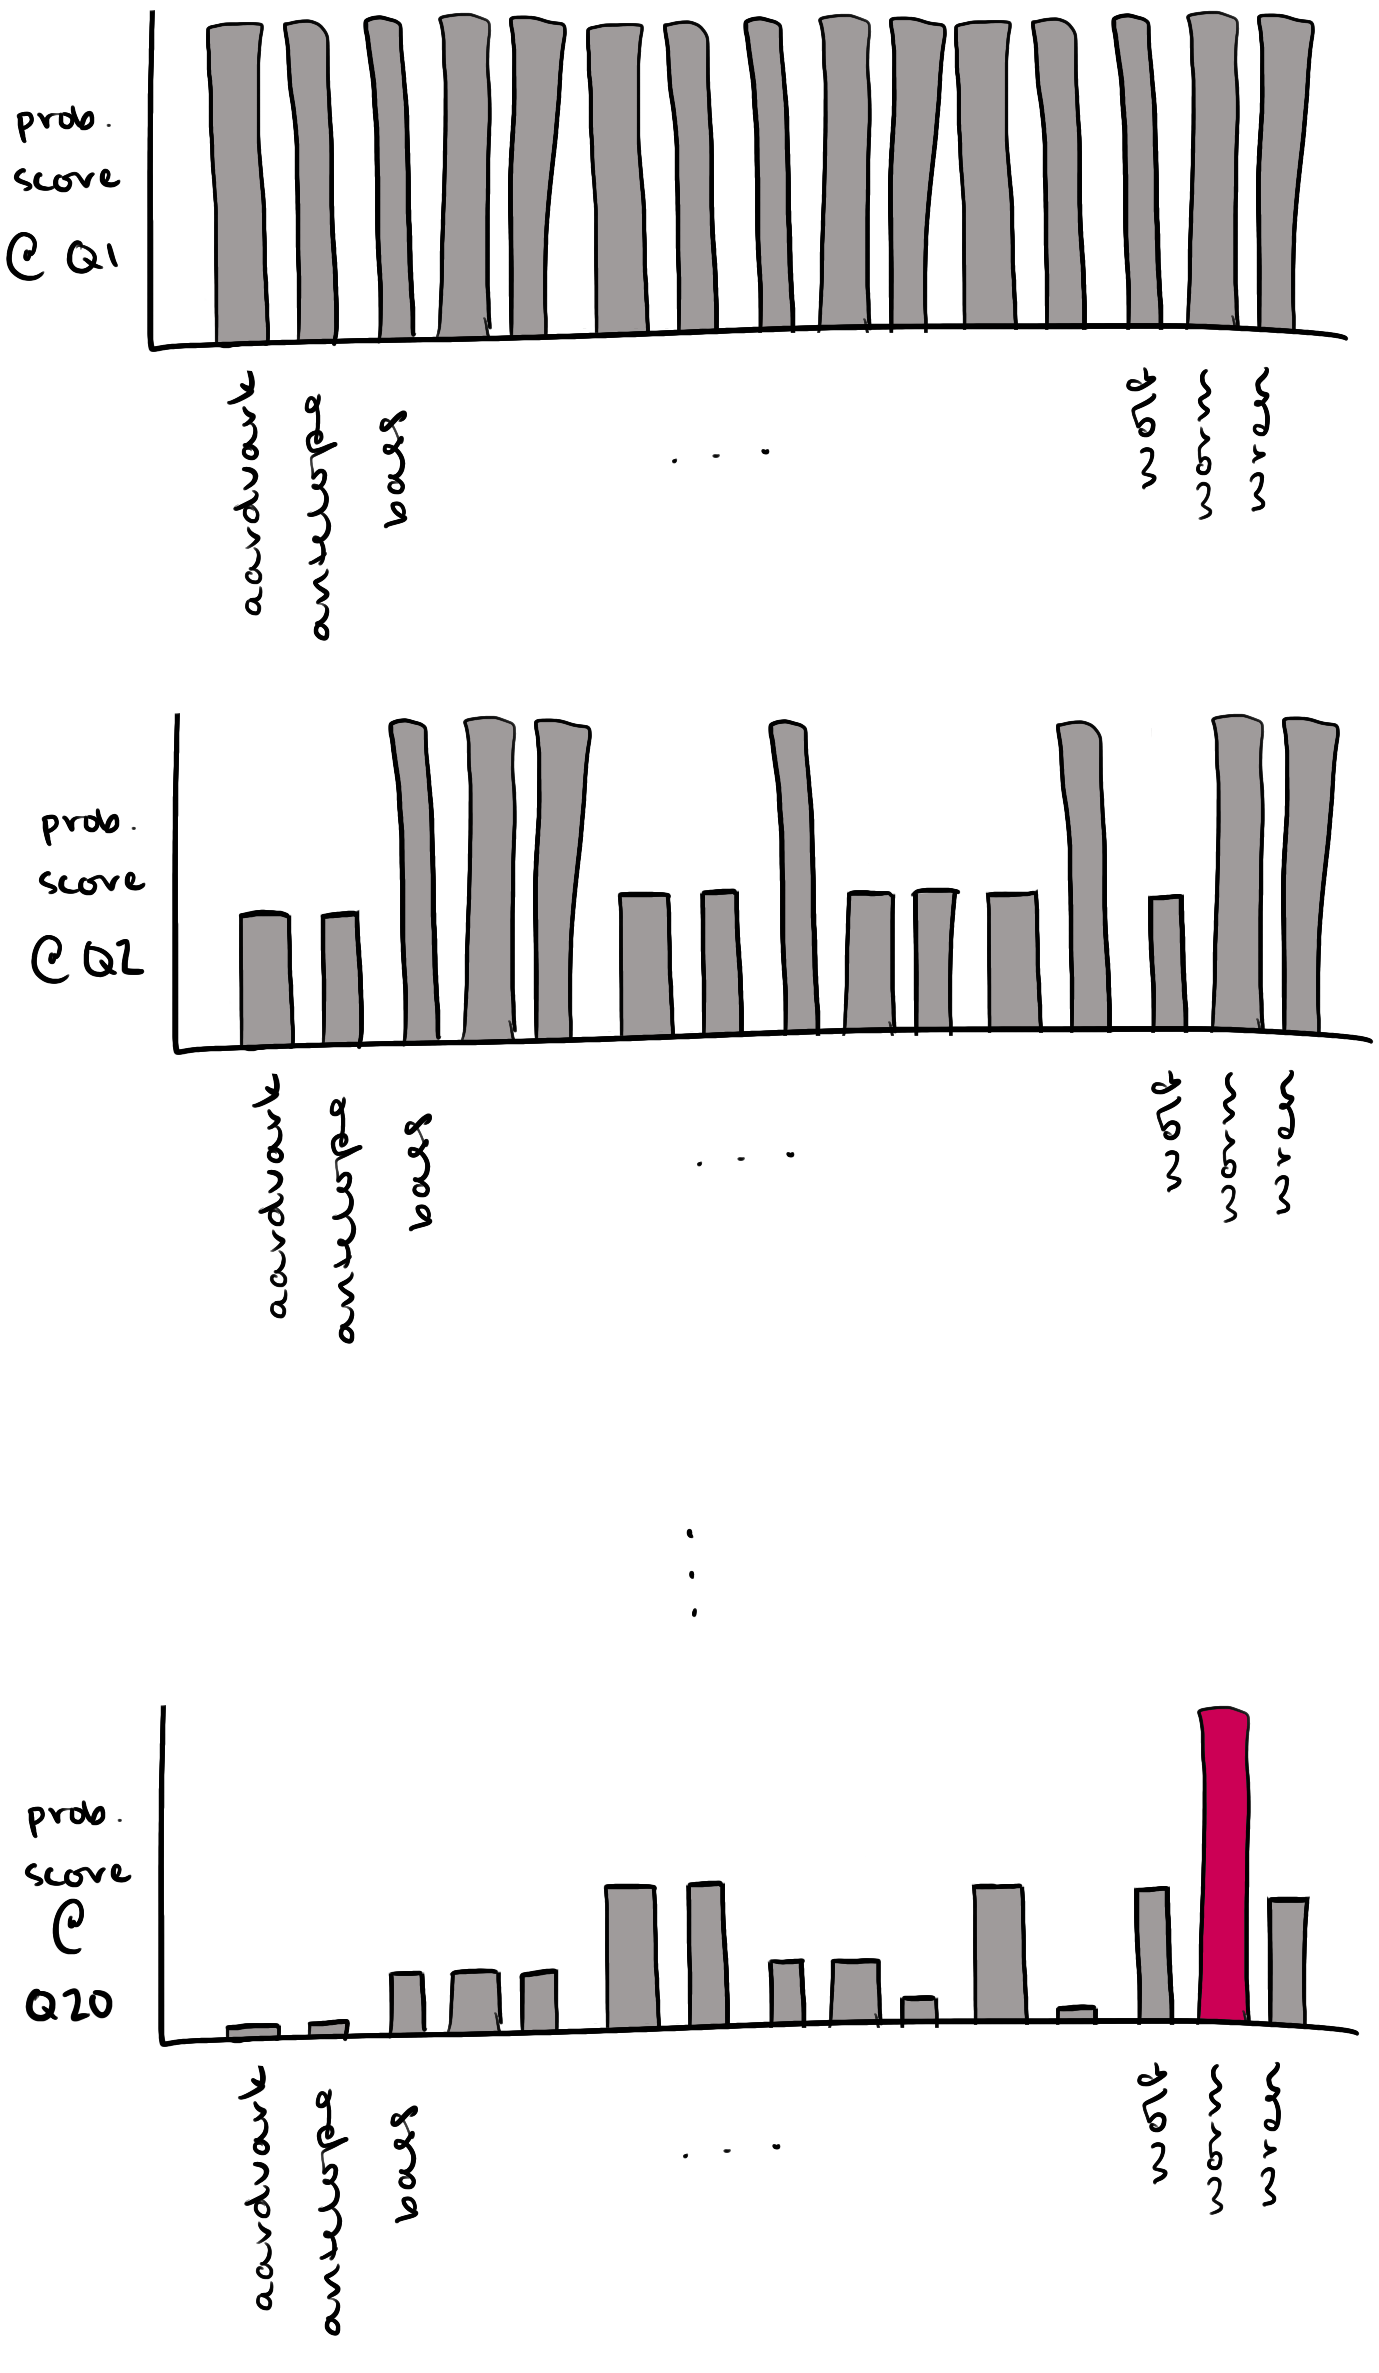
\includegraphics[width=.8\linewidth]{graphics/Bayesian-updating.png}
	\caption{Example distributions of probability scores across animals at Q1, Q2, and Q20, with the highest-probability animal (the one most consistent with the user's answers) highlighted}
	\label{fig:bayesian-update}
\end{figure}

\subsection{Rule-based question generation}

\lipsum[1]


\subsection{Incorporating out-of-database objects}

\lipsum[1]

``the perceived world is not an unstructured total set of equiprobable co-occurring attributes. Rather, the material objects of the world are perceived to possess (in Garner's 1974, sense) high correlational structure.
That is, given a knower who perceives the complex attributes of feathers, fur, and wings, it is an empirical fact provided by the perceived world that wings co-occur with feathres more than with fur'' \citep[29]{Rosch1978}

\section{Evaluation}

There is a straightforward measure of success of our system overall: $\frac{\text{games won}}{\text{games played}}$.
But because the system will (hopefully) consistently improve as we add new objects to its knowledge base, the success rates we get in early games with the system will presumably not be as good as success rates from later games. 
We can track this in a sort of growth curve across games:

\begin{center}
	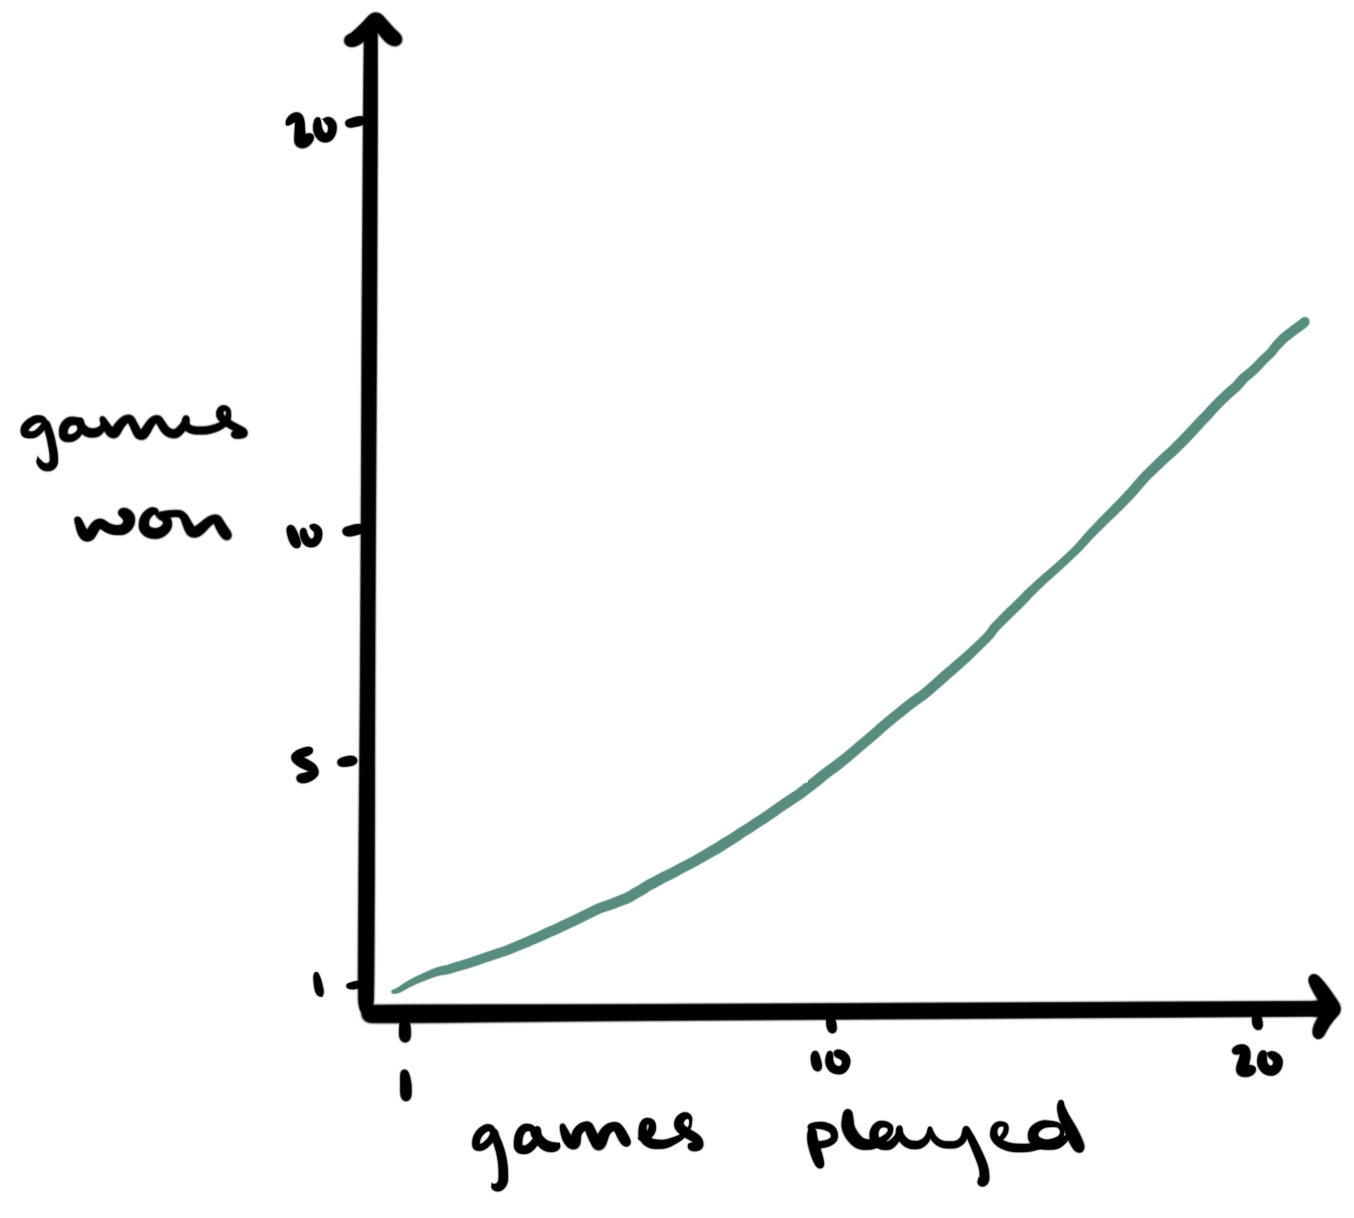
\includegraphics[width=.5\linewidth]{graphics/growth-curve.png}
\end{center}

The slope of the curve won't ever get bigger than one, but we'd want it to approach one, since that means the system is winning every game that it plays.
The slope of that curve at its endpoint is actually given by the rational expression $\frac{\text{games won}}{\text{games played}}$ \citep[50--51]{Baayen2001}, so we can evaluate how our system performs after some arbitrary number of games by looking at how close that value is to one.
Or alternately, we could look at $\frac{\text{games lost}}{\text{games played}}$ and see how close that value is to zero.
\begin{center}
	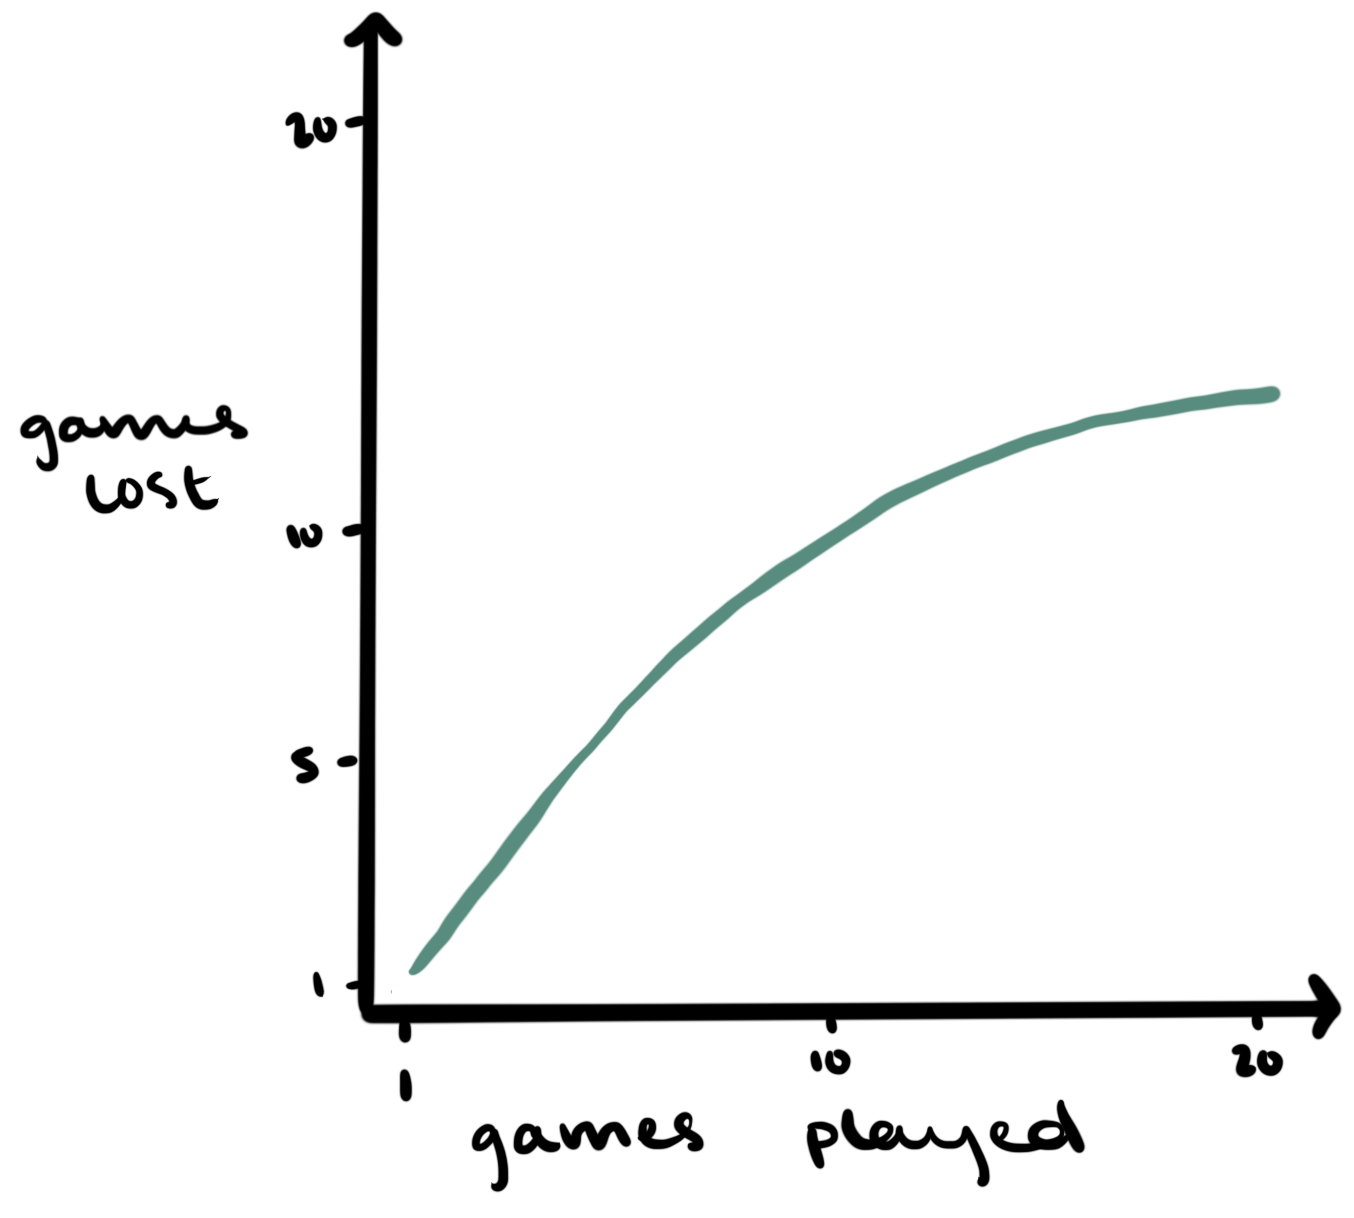
\includegraphics[width=.5\linewidth]{graphics/growth-curve2.png}
\end{center}

Depending on how intense we want to get, we could model this second growth curve using a Zipf-Mandelbrot model \citep{Evert2004}, and that would allow us to predict how many games our system would have lost after an arbitrarily large number of games played.
There is a package in R that we could use to do this: \texttt{zipfR} by \citet{BaroniEvert2014}.

(We should also keep track of whether/how many losses come from exceeding the twenty-question limit and how many come from out-of-database items. Ideally, the 20-question-limit curve will not change much, and the out-of-database curve would change more.
We should also keep track of the number of questions that it takes for the system to win.)

In addition to evaluating the system's performance in gameplay, we should also evaluate the goodness of the out-of-database items that we interpolate.
One way to do this would be to use ``crowdworkers'' (our friends, probably) to annotate the previously-unseen objects for all of the features that we use, and then compare those results to those output by the interpolation system.

\bibliography{qp}
\bibliographystyle{acl_natbib}

\appendix

\section{Individual contributions}
\label{app:contributions}

All group members were in regular, active communication about ideas and directions in which to take the project.
It was a fully collaborative effort throughout.
We summarise here how we divided the workload between the four of us.

\paragraph{Wellesley} Literature work, prepared and held the in-class presentation, wrote and proofread sections of the project plan and the final paper.

\paragraph{Anna} Literature work, implemented the question generation, wrote sections of the project plan and the final paper.

\paragraph{Rodrigo} Implemented the handling of out-of-database items, wrote sections of the final paper.

\paragraph{Elizabeth} Implemented the core functionalities of the game, wrote sections of the project plan and the final paper, hosted the GitHub repo, compiled \LaTeX\ files.

\end{document}
